\documentclass{article}
\usepackage{tikz}
\usetikzlibrary{decorations.pathmorphing}

\begin{document}

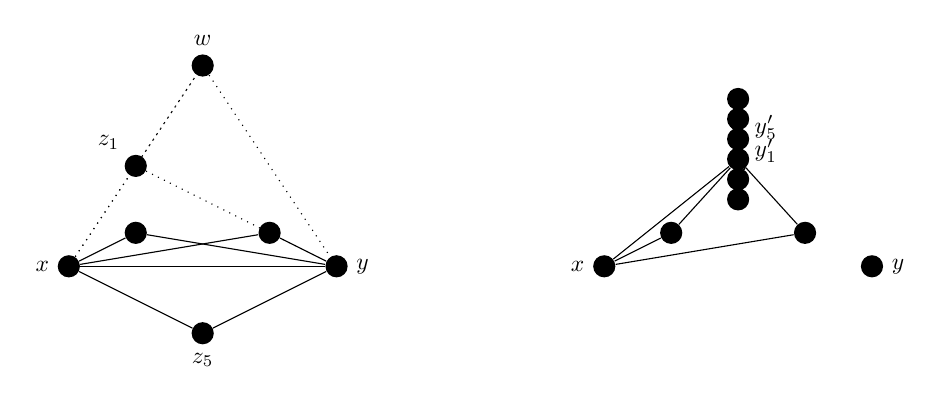
\begin{tikzpicture}[scale=0.85, transform shape]
    % Left graph
    \node[circle, fill=black, label=left:$x$] (x) at (0,0) {};
    \node[circle, fill=black, label=right:$y$] (y) at (4,0) {};
    \node[circle, fill=black, label=above:$w$] (w) at (2,3) {};
    \node[circle, fill=black, label=below:$z_5$] (z5) at (2,-1) {};
    \node[circle, fill=black, label=above left:$z_1$] (z1) at (1,1.5) {};
    
    % Connect nodes
    \draw (x) -- (y);
    \draw[dotted] (x) -- (z1) -- (y);
    \draw[dotted] (x) -- (w) -- (y);
    \draw[dotted] (z1) -- (w);
    \draw (x) -- (z5) -- (y);
    
    % Additional connections
    \foreach \i in {-1,1} {
        \node[circle, fill=black] (z\i) at (2+\i,0.5) {};
        \draw (x) -- (z\i) -- (y);
    }
    
    % Right graph
    \begin{scope}[xshift=8cm]
        \node[circle, fill=black, label=left:$x$] (x2) at (0,0) {};
        \node[circle, fill=black, label=right:$y$] (y2) at (4,0) {};
        
        % Central node connections
        \node[circle, fill=black] (c) at (2,1) {};
        \foreach \i in {1,...,5} {
            \node[circle, fill=black] (y\i) at (2,1+1.5*\i/5) {};
            \draw[decoration={coil,aspect=0}, decorate] (c) -- (y\i);
        }
        \node[label=above right:$y'_1$] at (y1) {};
        \node[label=below right:$y'_5$] at (y5) {};
        
        % Connect outer nodes
        \draw (x2) -- (y2);
        \foreach \i in {-1,1} {
            \node[circle, fill=black] (z\i) at (2+\i,0.5) {};
            \draw (x2) -- (z\i) -- (y2);
        }
    \end{scope}
\end{tikzpicture}

\end{document}